\chapter{Objetivos}
\label{cap:objetivos}

El objetivo global de este proyecto \textbf{OBJ-G} es desarrollar un sistema completo y libre de \textbf{enfoque} astronómico. Dicho sistema debe permitir un modo de funcionamiento remoto utilizando el protocolo \textbf{INDI}.


\bigskip
Este objetivo global se desglosa en los siguientes objetivos principales:

\begin{itemize}
  \item \textbf{OBJ-P1.} Diseño dispositivo hardware, usando plataforma libre \textbf{Arduino},
  que interactúe directamente con los mandos de enfoque del \textbf{telescopio}, mediante un motor y distintos sensores.
  \item \textbf{OBJ-P2.} Implementar un firmware, que permita realizar el control de todos los periféricos y electrónica.
  \item \textbf{OBJ-P3.} Implementar un \textbf{Driver INDI} que provea de la funcionalidad básica para controlar
   todas las características o propiedades del dispositivo enfocador.
  \item \textbf{OBJ-P4.} Diseñar un algoritmo de autofocus, basándonos en una medida del foco y coordinada con las funciones del dispositivo y las imágenes capturadas por una CCD \textit{[opcional, puesto que ya existen soluciones software que lo hacen usando INDI]}.

\item \textbf{OBJ-P5.} Documentar y difundir extensivamente el trabajo para que sea reproducible por todos los interesados.

\end{itemize}


\bigskip
Dado los objetivos principales del proyecto, podemos hacer un desglose en objetivos menores, separándolos a su vez en objetivos  \textbf{Obligatorios}, que deben cumplirse para llegar a completar su correspondiente objetivo principal, y objetivos \textbf{Secundarios}, objetivos igualmente interesantes para el proyecto, pero que carecen de importancia vital y su incumplimiento no evita que se pueda completar su correspondiente objetivo central.
\newpage

\begin{itemize}
  \item \textbf{OBJ-P1.O1.}  Investigación de los periféricos y sensores existentes para la plataforma Arduino,
  \item \textbf{OBJ-P1.O2.}  Realizar una estimación de precios y gastos en componentes, sopesando distintas alternativas.
  \item \textbf{OBJ-P1.O3.}  Investigar sobre los distintos métodos de mecanización para los materiales empleados, así como posibles alternativas para crear la PCB y carcasas del dispositivo.
  \item \textbf{OBJ-P1.O4.}  Implementar un prototipo completo.
  \item \textbf{OBJ-P1.S1.}  Implementación de distintas versiones, completa, solo funcionamiento remoto o solo control manual.
\end{itemize}



\begin{itemize}
  \item \textbf{OBJ-P2.O1.} Investigar librerías de control de los periféricos, buscando alternativas y realizando pruebas y ejemplos.
  \item \textbf{OBJ-P2.O2.} Implementar un \textbf{Firmware}, basándonos en un diseño modular, permitiendo así que futuras ampliaciones sea fáciles.
  
  \begin{itemize}
  	\item \textbf{OBJ-P2.O2.M1} Módulo de control de motores paso a paso.
  	\item \textbf{OBJ-P2.O2.M2} Módulo visualización de datos en pantalla LCD.
  	\item \textbf{OBJ-P2.O2.M3} Módulo control manual.
  	\item \textbf{OBJ-P2.O2.M4} Módulo control remoto y comunicación con host.
  	\item \textbf{OBJ-P2.O2.M4} Módulo de sensores externos.
  \end{itemize}
  
 
  \item \textbf{OBJ-P2.O3.} Definir protocolo de comunicación, mensajes y parámetros, entre ordenador y el dispositivo.

  \item \textbf{OBJ-P2.O4.} Realizar las pruebas pertinentes para comprobar el buen comportamiento de la lógica, sobre la electrónica previamente diseñada, así como la integración de los distintos módulos.
  \item \textbf{OBJ-P2.S1.} Implementar protocolo de intercambio de mensajes \textbf{Robofocus} (sección~\ref{sec:robofocus}).
\end{itemize}


\begin{itemize}
  \item \textbf{OBJ-P3.O1.} Que cumpla el entandar INDI para enfocadores
  \item \textbf{OBJ-P3.S1.} Que el driver proporcione información sobre los sensores.
  \item \textbf{OBJ-P3.S2.} Realizar script de despliegue automatizado, para instalar y correr el Servidor INDI con su correspondiente driver.
\end{itemize}


\begin{itemize}
  \item \textbf{OBJ-P4.O1} Implementar un pequeño framework de visualización y procesamiento de imágenes, que permita evaluar y parametrizar de forma simple los algoritmos que aplicamos sobre las imagenes estelares.
  \item \textbf{OBJ-P4.S2} Diseño y implementación de algoritmos de detección de objetos celestes, con propiedades estelares, basándonos en la curva de luz característica.
  \item \textbf{OBJ-P4.O3} Realizar cálculo de distintas medidas de enfoque, calculo del FWHM.
  \item \textbf{OBJ-P4.S4} Dada la medida anterior, implementar algoritmos de búsqueda de máximo enfoque, coordinado con el movimiento del enfocador y la adquisición de las imagenes por parte de la CCD.

\end{itemize}

\bigskip
Además de los objetivos anteriores, se persigue alcanzar los siguientes objetivos secundarios globales:

\begin{itemize}
  \item \textbf{OBJ-P5-O1.} Completar una buena documentación técnica, así como información variada para desarrolladores, a fin de que cualquier interesado sea capaz de reproducir fácilmente y a bajo costo el proyecto.
  \item \textbf{OBJ-P5-O2.} Publicar código fuente, diseños y documentación bajo una licencia libre (GNU3 o similar), que permita que la comunidad de desarrolladores interesados pueda realizar modificaciones y personalizaciones.
  \item \textbf{OBJ-P5-S1.} Difusión en la comunidad astronómica y desarrollo de una web propia del proyecto.
\end{itemize}

Estos objetivos se han representado gráficamente en la figura~\ref{fig:objetivos}.

\begin{figure}
\centering
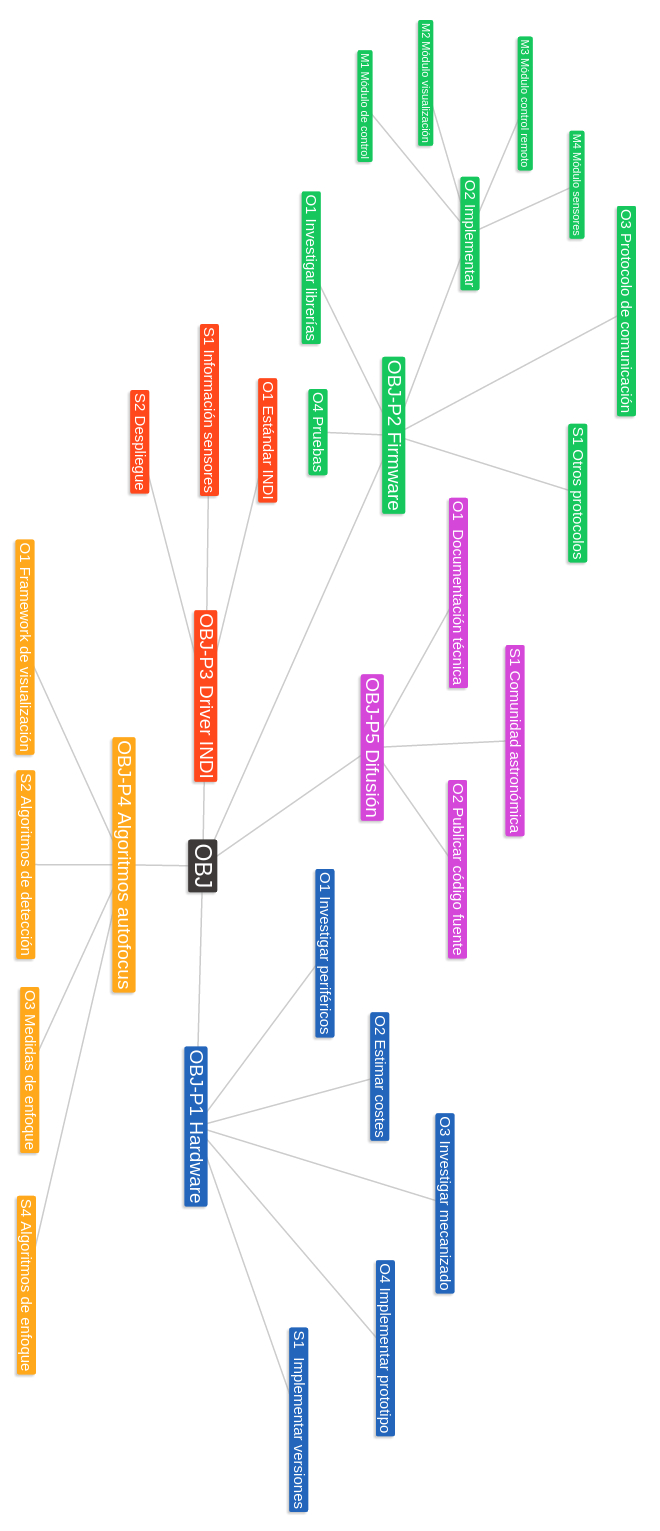
\includegraphics[width=0.7\linewidth]{../images/diagrama_objetivos}
\caption[Diagrama de los Objetivos del Proyecto]{Diagrama de los Objetivos del Proyecto}
\label{fig:objetivos}
\end{figure}


Para la realización de los objetivos se pondrán en práctica los conocimientos alcanzados en las siguientes materias impartidas en la Escuela Técnica Superior de Ingenierías Informática y de Telecomunicación de la Universidad de Granada:

\begin{itemize}
  \item \textbf{Ingeniería del software} para el análisis y diseño del proyecto, así como modelar el sistema.
  \item \textbf{Programación orientada a objetos} para la estructura y la organización del código \textbf{Java}.
  \item \textbf{Programación de sistemas multimedia} para poder implementar las interfaces de usuario en \textbf{Java Swing}, así como visualizar y tratar las imágenes.
  \item \textbf{Infraestructuras virtuales} para poder gestionar los sistemas, teniendo habilidad para realizar instalaciones y aprovisionamiento en servidores.
  \item \textbf{Transmisión de datos y redes de computadores} para comprender  el funcionamiento de las capas de red y los puertos, base para comprender el protocolo \textbf{INDI} y configurar correctamente las redes para las pruebas.
  \item \textbf{Algorítmica} para optimizar las rutinas de tratamiento de imágenes.
  \item \textbf{Calculo matemático} para poder implementar las funciones matemáticas necesarias. 
  \item \textbf{Estructura de datos} para modelar la representación de las imágenes de una forma eficiente.
  \item \textbf{Tecnologías Emergentes} para conocer las plataformas de hardware libre y domótica. 
\end{itemize}

\bigskip
Por otro lado, han sido necesarios alcanzar conocimientos en otras áreas:

\begin{itemize}

  \item \textbf{Astronomía básica y equipos astronómicos} para entender a los usuarios potenciales y poder acomodar la aplicación a sus necesidades.
  \item \textbf{Electrónica básica y Arduino} para diseñar y construir dispositivo hardware. 
  \item \textbf{Raspberry Pi} para montar un servidor permanente de pruebas o acceso público para probar la aplicación. 
  \item \textbf{\LaTeX} para la realización del presente documento y la ampliación de conocimientos para futuros textos científicos.
  \item \textbf{Git} para la gestión de versiones y la publicación de código abierto que permita a otros desarrolladores participar.
\end{itemize}
